Murtolukujen lisäksi desimaaliluvut ovat tuttu tapa merkitä lukuja, jotka eivät ole kokonaislukuja.

$123,456$ on esimerkki desimaaliluvusta. Pilkun jälkeen tulevat numerot tarkoittavat kymmenesosia, sadasosia ja niin edelleen.

\begin{alakohdat}
	\alakohta{$123$ on sen \termi{kokonaisosa}{kokonaisosa}.}
	\alakohta{Kokonaisluku erotetaan loppuosasta \termi{desimaalierotin}{desimaalierottimella}, joka on suomen kielessä pilkku (,)}
	\alakohta{Osaa $456$ kutsutaan luvun \termi{desimaaliosa}{desimaaliosaksi}.}
\end{alakohdat}

\laatikko{

Esimerkkinä annettu desimaaliluku tulkitaan seuraavasti:
\begin{equation*}
123,456 = 1 \cdot 10^2 + 2 \cdot 10^1 + 3 \cdot 10^0 + 4 \cdot 10^{-1} + 5 \cdot 10^{-2} + 6 \cdot 10^{-3}
\end{equation*}

\begin{equation*}
\huge \bf \underbrace{1}_{1\cdot10^2}\underbrace{2}_{2 \cdot 10^1}\underbrace{3}_{3 \cdot 10^0},\underbrace{4}_{4 \cdot 10^{-1}}\underbrace{5}_{5 \cdot 10^{-2}}\underbrace{6}_{6 \cdot 10^{-3}}
\end{equation*}

\begin{center}
 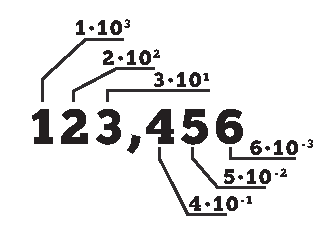
\includegraphics{pictures/Kuva5-1-desimaali-potenssit.pdf}
\end{center}
}

Kymmenjärjestelmä saa nimensä siitä, että jokainen luvussa esiintyvä numeromerkki kertoo sen paikkaa vastaavien kymmenen potenssien määrän.

\subsubsection*{Murtoluvun muuttaminen desimaaliluvuksi}

Murtoluku on tapa merkitä jakolaskua. Jakolaskun tuloksen esittämiseksi desimaalilukuna
käytetään peruskoulun alaluokilla opetettavaa jakokulmaa. Jakokulman ajatus on yksinkertaisesti kokeilla, kuinka monta jakajaa, sen kymmenesosaa, sadasosaa ja niin
edelleen jaettavaan mahtuu. Jakokulmat voi laskea käsin, laskin tekee saman nopeammin.

\begin{esimerkki}
Muutetaan $\frac{21}{4}$ desimaaliluvuksi laskemalla jakolasku $21 : 4$ jakokulmassa.
% Voisiko laskuun selitää myös sanallisen selityksen siitä, mitä missäkin vaiheessa tapahtuu? Esim.
% Huomataan että luku 4 menee lukuun 21 viisi kertaa -> merkitään 5 jakokulman yläpuolelle ykkösten kohdalle.
% Tarkistetaan jakolasku kertolaskun avulla: $4 \cdot 5 = 20$. 
% Lasketaan jakojäännös erotuksena $21 - 20 = 1$.
% Luku 4 ei mene lukuun 1 yhtään kertaa, joten ``pudotetaan'' jaettavasta 0 desimaalierottimen oikealta puolelta (vastaukseen pitää muistaa merkitä desimaalierotin vastaavaan kohtaan kuin jaettavassa.) Luku 4 menee lukuun 10 kaksi kertaa -> merkitään 2 jakokulmaan kymmenesosien kohdalle.
% Tarkistetaan jakolasku kertolaskun avulla: $4 \cdot 2 = 8$, ja jakojäännökseksi jää $10 - 8 = 2$.
% ...
%
%
% Kun jakojäännökseksi jää luku nolla, jako on mennyt tasan ja vastaus on luettavissa jakokulman yläpuolelta.



\[ 
\begin{array}{cccccc}
 & \underline{ \ \ } & \underline{5}, & \underline{2} & \underline{5} \\
 4 & \!\!|\,2 & 1, & 0 & 0 \\
 \underline{-} & \underline{2}& \underline{0} \\
 & & 1 &0 \\
 & \underline{-} &\underline{ \ \ }  & \underline{8} \\
 & & & 2 & 0 \\
 & & \underline{-} & \underline{2} & \underline{0} \\
 & &  & & 0
\end{array}
\]
Siis $\dfrac{21}{4} = 5,25$.


Vastaavasti laskien saadaan $\dfrac{3}{11}=0,272727\ldots \ $ :
\[ 
\begin{array}{cccccc}
 & \underline{ 0}, & \underline{2} & \underline{7} & \underline{2} & 
 \underline{\ldots} \\
 11 & \!\!|\,3, & 0 & 0 & 0 & \ldots \\
 \underline{-} & \underline{2}& \underline{2} \\
 & & \boldsymbol{8} &0 \\
 & \underline{-} &\underline{ 7 }  & \underline{7} \\
 & & & \boldsymbol{3} & 0 \\
 & & \underline{-} & \underline{2} & \underline{2} \\
 & &  & & \boldsymbol{8} & 0 \\
 & & & & & \ddots
\end{array}
\]
Koska jakojäännökset 3 ja 8 toistuvat loputtomiin, tämä desimaaliluku
ei ole päättyvä. Siinä on \termi{jakso}{jakso}: numerosarja 27 toistuu.
Jaksoa voidaan merkitä yläviivan avulla seuraavasti:
\[ 0,27272727\ldots = 0,\overline{27} \]
\end{esimerkki}

{\bf Kaikkien murtolukujen desimaaliesitykset ovat joko päättyviä tai jaksollisia.}
Vähennyslaskuissa syntyvät jakojäännökset ovat nimittäin aina jakajaa pienempiä, ja siksi
ne alkavat väistämättä toistaa itseään, ellei jako jossakin vaiheessa mene tasan.
Koska eri vaihtoehtoja jakojäännöksiksi on yksi jakajaa vähemmän,
jakson pituus on suurimmillaan yhden verran jakajaa pienempi. Esimerkiksi luvulla
$\dfrac{1}{7}=0,\overline{142857}$ jakso on pisin mahdollinen, $7-1=6$ numeron mittainen.

\laatikko{
Tässä on joitain murtolukujen desimaaliesityksiä, jotka on hyvä osata
\begin{alakohdat}
	\alakohta{$ \frac{1}{10} = 0,1$}
	\alakohta{$ \frac{1}{100} = 0,01$}
	\alakohta{$ \frac{1}{2} = 0,5$}
	\alakohta{$ \frac{1}{4} = 0,25$}
	\alakohta{$ \frac{3}{4} = 0,75$}
\end{alakohdat}
}

\subsubsection*{Desimaaliluvun muuttaminen murtoluvuksi}

\termi{päättyvä desimaaliluku}{Päättyvät desimaaliluvut} voidaan muuttaa murtoluvuiksi muuttamalla kukin
desimaali erikseen murtoluvuksi ja laskemalla syntyneet luvut yhteen.

\begin{esimerkki}
$21,37 = 21+ \frac{3}{10}+\frac{7}{100} =
\frac{2100}{100}+\frac{30}{100}+\frac{7}{100}
 = \frac{2100+30+7}{100} = \frac{2137}{100}.$
\end{esimerkki}

Tämä on turhan työlästä, ja paljon helpommalla päästäänkin kun lavennetaan luku ''niin monella kympillä, kuin siinä on numeroita desimaalipilkun jälkeen''. Täsmällisemmin sanottuna luvulla $10^n$, jossa $n$ on pilkun jälkeen tulevien numeroiden määrä.

\begin{esimerkki}
$21,47 = 21,37 \cdot  \frac{100}{100} = \frac{21,37 \cdot 100}{100} = \frac{2137}{100}$
\end{esimerkki}

\begin{esimerkki}
$0,007 = 0,007 \cdot 1 = 0,007 \cdot \frac{10^3}{10^3} = \frac{0,007 \cdot 1000}{1000} = \frac{7}{1000}$

\end{esimerkki}

%Menetelmän toimivuus kaikkien desimaalilukujen tapauksessa voidaan todistaa %tarkastelemalla desimaaliluvun määritelmää, mutta jätetään tässä tekemättä.

Minkä tahansa \termi{jaksollinen desimaaliluku}{jaksollisen desimaaliluvun} voi muuttaa murtoluvuksi seuraavalla tempulla.
Muutetaan esimerkiksi $0,575757\ldots$ murtoluvuksi. Jos merkitään
\[
\begin{array}{rcll}
x &=& \ \, 0,575757 \ldots\ , &\textrm{saadaan sadalla kertomalla} \\
100x &=& 57,575757 \ldots \ , &\textrm{joiden erotuksena} \\
100x - x &=& 57,57 \ldots - 0,57 \ldots \ , & \textrm{eli} \\
99x &=& 57, & \textrm{josta saadaan} \\
x &=& \frac{57}{99} = \frac{19}{33}.
\end{array}
\]
Siis $0,575757\ldots = \frac{19}{33}$. Menetelmä toimii kaikille jaksollisille
desimaaliluvuille: kerrotaan vain sopivalla luvun 10 potenssilla, jotta jakso
katoaa vähennyslaskussa.

\laatikko{
Nämä kannattaa muistaa:
\begin{alakohdat}
	\alakohta{$ \frac{1}{3} = 0,3333 \ldots$}
	\alakohta{$ \frac{2}{3} = 0,6666 \ldots$}
\end{alakohdat}
}
